\documentclass{article}

\title{Assignment 3 : CS215}
\author{Akshat Chugh : 170050019 \\ Satvik Ambati : 170050101}
\usepackage{amsmath}
\usepackage{amssymb}
\usepackage{enumerate}
\usepackage{graphicx}
\usepackage[margin=0.5in]{geometry}
\begin{document}
\maketitle
\begin{enumerate}
	\setcounter{enumi}{1}
	\item $X \sim U(0,1)$ \\
	Let $Y = g(X)$ \\
	$\implies X = g^{-1}(Y)$ 
	\begin{align}
	y &= \frac{-1}{\lambda} log(x) \\
	\implies  x &=  e^{-\lambda y}
	\end{align}
	$$  \Big| \frac{d}{dy} g^{-1}(y) \Big| = \lambda e^{-\lambda y}$$
	Let PDF of $Y$ be denoted by $q(y)$ and the PDF of $X$ by $p(y)$ .
	$$ \implies q(y) = \Big| \frac{d}{dy} g^{-1}(y) \Big| p(g^{-1}(y)) = \lambda e^{-\lambda y}$$
	Therefore, the transformed data $Y$ will have an \textbf{exponential distribution} with $mean = \frac{1}{\lambda}$. \\
	\\ Given :
	\begin{itemize}
		\item $\lambda = 5$
		\item Gamma prior with parameters $\alpha = 5.5$ and $\beta = 1$
	\end{itemize}
	\textbf{MLE for exponential distribution:} \\
	The likelihood function is : 
	$$L(\lambda; x_1, x_2,...,x_n) = \lambda^n exp( - \lambda \sum_{j=1}^{n} x_j)$$
	The log likelihood function is :
	$$ l(\lambda, x_1, x_2,...,x_n) = n ln(\lambda) - \lambda \sum_{j=1}^{n} x_j$$
	Therefore, the maximum likelihood estimator of $\lambda$ is the reciprocal of the sample mean ( $\frac{\sum_{j=1}^{n} x_j}{n}$)
	$$\hat{\lambda} = \frac{n}{\sum_{j=1}^{n} x_j}$$ \\
	\textbf{Bayesian Posterior Mean Estimator:}
	$$ Prior: \ P(\theta) = \ Gamma(\lambda | \alpha, \beta) \propto \lambda^{\alpha - 1} exp(-\beta \lambda) $$ 
	\begin{align*}
	P(\theta | x_1,x_2,...,x_n) &\propto P(x_1,x_2,...,x_n | \theta) \ P(\theta) \\
	&\propto \lambda^{n} \ exp(- \lambda \sum_{j=1}^{n} y_j) \ \lambda^{\alpha - 1} \ exp(-\beta \lambda)
	\\ &\propto \lambda^{n+\alpha-1} \ exp(- \lambda (\beta + \sum_{j=1}^{n} y_j)) \\
	&\propto \ Gamma(\lambda | \alpha + n, \beta + \sum_{j=1}^{n} y_j)
	\end{align*}
	We know that, mean of a Gamma distribution with parameters $\alpha$ and $\beta$ is $\frac{\alpha}{\beta}$. \\
	We also know that Bayesian Posterior mean estimator = $E_{P(\theta | x_1,x_2,...,x_n)} [\theta]$
	$$\implies E_{P(\theta | x_1,x_2,...,x_n)} [\theta] = \ Mean \ of \ Gamma(\lambda | \alpha + n, \beta + \sum_{j=1}^{n} y_j)$$
	$$\implies E_{P(\theta | x_1,x_2,...,x_n)} [\theta] = \frac{\alpha + n}{\beta + \sum_{j=1}^{n} y_j}$$
	$$ \therefore \hat{\lambda}^{PosteriorMean} = \frac{\alpha + n}{\beta + \sum_{j=1}^{n} y_j}$$
	\begin{center}
		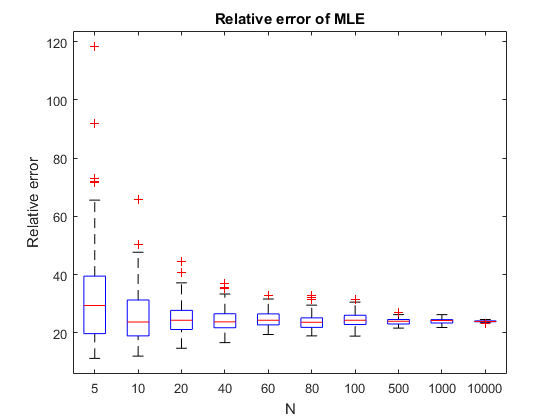
\includegraphics[scale=0.8]{p2_mle} \\
		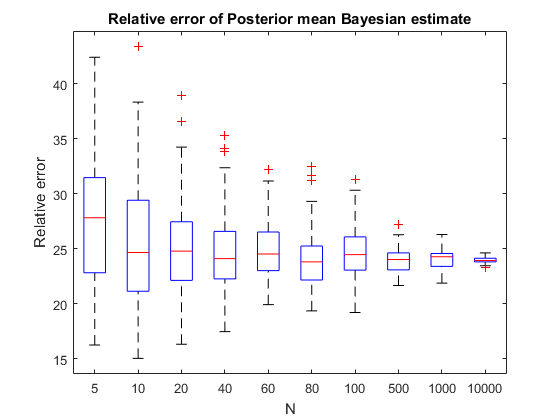
\includegraphics[scale=0.8]{p2_bpme} \\
		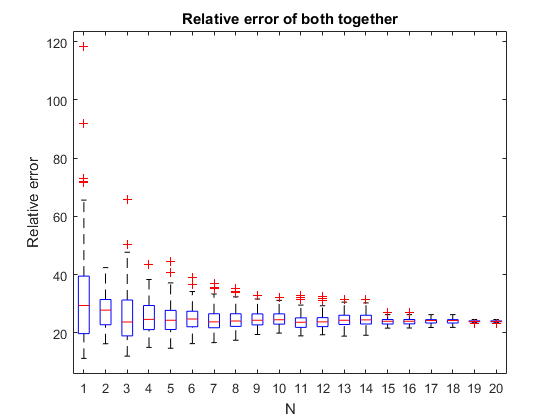
\includegraphics[scale=0.8]{p2_both} \\
	\end{center}
	In the above plot, every alternate box starting with the first denotes the relative error plot of MLE and the other set of alternate boxes starting with the second denotes the relative error plot of Bayesian Posterior mean estimate.
	$$  \hat{\lambda}^{PosteriorMean} = \frac{\alpha + n}{\beta + \sum_{j=1}^{n} y_j}$$
	$$ \hat{\lambda}^{PosteriorMean} = \Big(\frac{\alpha}{\beta}\Big) \Big(\frac{\beta}{\beta + \sum_{j=1}^{n} y_j}\Big) + \Big(\frac{n}{\sum_{j=1}^{n} y_j}\Big) \Big(\frac{\sum_{j=1}^{n} y_j}{\beta + \sum_{j=1}^{n} y_j}\Big)$$
	
	$$\hat{\lambda}^{PosteriorMean} = \Big(\frac{\alpha}{\beta}\Big) w + \Big(\frac{n}{\sum_{j=1}^{n} y_j}\Big) (1-w) \ \ \ where \ w = \Big(\frac{\beta}{\beta + \sum_{j=1}^{n} y_j}\Big)$$
	
	\begin{enumerate}[(i)]
		\item As the value of $n$ increases, the     relative error for MLE and Bayesian Posterior Mean Estimate does not follow a strict pattern but may increase or decrease or both.\\
		For very large $n$, as the Bayesian Posterior Mean Estimate tends to the Maximum Likelihood estimate, the relative error of Bayesian Posterior mean estimate also tends to the relative error of the maximum likelihood estimate.
		\item Any of the two estimates may be taken 
	\end{enumerate}
\end{enumerate} 
\end{document}